\documentclass[a4paper,12pt,oneside]{article}
%%% Escrever em Português
%%%%%%%%%%%%
\usepackage[brazil]{babel}
\usepackage[utf8]{inputenc}
\usepackage[T1]{fontenc}
%%% Usando referencias para footnotes
\usepackage{footmisc}
%%% Cores para os footnotes
%\usepackage{xcolor}
\usepackage[usenames,dvipsnames]{xcolor}
%%% Cores em tabelas
\usepackage{color, colortbl}

%%% Escolha das fontes
%%% Combo: Palatino + Helvetica + Courier, com EulerVM para matemática
\usepackage{mathpazo}
\usepackage[scaled=.95]{helvet}
\usepackage{courier}
\linespread{1.05} %%% Palatino needs more spacing.
%%% Geometria da página. Sugiro manter estas mesmas margens e 15 cm de espaço de texto.
%\usepackage[a4paper,pdftex,top=2.8cm,bottom=4cm,left=3.4cm,right=2.6cm]{geometry}
%\textwidth=15.0 true cm

% Hide subsubsections
%\setcounter{secnumdepth}{2}
%\setcounter{tocdepth}{2}

\usepackage{sprace}
\usepackage{multirow} % allowing to merge rows in table
% Use isto pros headers
\usepackage{fancyhdr}
%\setlength{\headheight}{15.2pt}
%\pagestyle{fancy}
%\renewcommand{\chaptermark}[1]{\markboth{\chaptername\ \thechapter.\ #1}{}}
%% E menos espaço ao começar o capítulo
\usepackage{titlesec}
\titleformat{\chapter}[display]
  {\normalfont\rmfamily\huge\mdseries}
  {\chaptertitlename\ \thechapter}{20pt}{\huge}
\titlespacing*{\chapter}{0pt}{-20pt}{40pt}
% Linha Extra
\newcommand{\linha}{\enlargethispage{1\baselineskip}}
% Páginas bonitas
\fancypagestyle{plain}{%
\fancyhf{} % clear all header and footer fields
\fancyfoot[C]{\textit \thepage} % except the center
\renewcommand{\headrulewidth}{0pt}
\renewcommand{\footrulewidth}{0pt}}
\fancypagestyle{fancyplain}{%
\fancyhf{}
\fancyhead[L]{\textit{\leftmark}}
\fancyhead[R]{\textit{\thepage}}
%%%%%\fancyfoot[C]{\today} % Use este fancyfoot pros drafts (data no pé da página)!
\fancyfoot[C]{} % Use este fancyfoot (vazio) pra versão final!
\renewcommand{\headrulewidth}{0.6pt}
\renewcommand{\footrulewidth}{0pt}}

%%%%%%%%%%%% Colorindo footnot marks %%%%%%%%%%%%%%%%%%%%%%%%%%%%%%%%%%%%%%%%%%
\renewcommand\thefootnote{\textcolor{blue}{\arabic{footnote}}}

%%%%%%%%%%%% Colorindo tabelas %%%%%%%%%%%%%%%%%%%%%%%%%%%%%%%%%%%%%%%%%%%%%%%%

%\newcommand{\Ab}{\cellcolor{blue}\phantom{x}}
%\newcommand{\Ag}{\cellcolor{gray}\phantom{x}}
%\newcommand{\Av}{\cellcolor{green}\phantom{x}}
%\newcommand{\Ar}{\cellcolor{red}\phantom{x}}
%\newcommand{\Aw}{\cellcolor{white}\phantom{x}}
%\newcommand{\Ab}{\multirow{2}{*}{x}}
%\newcommand{\Ag}{\multirow{2}{*}{x}}
%\newcommand{\Av}{\multirow{2}{*}{x}}
%\newcommand{\Ar}{\multirow{2}{*}{x}}
%\newcommand{\Aw}{}
%\newcommand{\Ab}{\multirow{2}{*}{\cellcolor{blue}\phantom{x}}}
%\newcommand{\Ag}{\multirow{2}{*}{\cellcolor{gray}\phantom{x}}}
%\newcommand{\Av}{\multirow{2}{*}{\cellcolor{green}\phantom{x}}}
%\newcommand{\Ar}{\multirow{2}{*}{\cellcolor{red}\phantom{x}}}
%\newcommand{\Aw}{}
\newcommand{\Ab}{\multirow{2}{*}{\bf \color{Black}{\#}}}
\newcommand{\Ag}{\multirow{2}{*}{\bf \color{Orange}{\#}}}
\newcommand{\Av}{\multirow{2}{*}{\bf \color{Cyan}{\#}}}
\newcommand{\Ar}{\multirow{2}{*}{\bf \color{red}{\#}}}
\newcommand{\Ap}{\multirow{2}{*}{\bf \color{PineGreen}{\#}}}
\newcommand{\Aw}{}


%%%%%%%%%%%% Comandos para facilitar a vida %%%%%%%%%%%%%%%%%%%%%%%%%%%%%%%%%%%
\newcommand{\pt}{\ensuremath{p_{_T}}}
\newcommand{\ptone}{\ensuremath{p_{T1}}\hspace{0.1cm}}
\newcommand{\pttwo}{\ensuremath{p_{T2}}\hspace{0.1cm}}
\newcommand{\muOne}{\ensuremath{\mu_{1}}\hspace{0.1cm}}
\newcommand{\muTwo}{\ensuremath{\mu_{2}}\hspace{0.1cm}}
\newcommand{\dzero}{D\O}
\newcommand{\DZERO}{\dzero}
\renewcommand{\trigger}{{\it trigger}}
\newcommand{\triggers}{{\it triggers}}
\newcommand{\nicefrac}[2]{\raise.5ex\hbox{\footnotesize #1}\kern-.15em/\kern-.15em\lower.25ex\hbox{\footnotesize #2}}
%\hypersetup{pdftitle={Procura de Sinais de Dimensões Extras Universais em Colisões Próton-Antipróton},
%            pdfauthor={Angelo de Souza Santos},
%            pdfsubject={High Energy Physics},
%            pdfkeywords={High Energy Physics}
%            			{Particle Physics}
%            			{Hadron Colliders} 
%				{Extra Dimensions}
%				{Beyond the Standard Model},
%			colorlinks=true,
%			citecolor=blue,
%			linkcolor=blue			
%            }
%\begin{document}
%%% This makes all the frontmatter stuff, sans the Table of Contents.
%\pagestyle{plain}
%\include{Preambulo}
%%%% The Table of Contents and a new page
%\tableofcontents
%\newpage
%\pagestyle{fancyplain}
%%\pagestyle{headings}
%\pagenumbering{arabic}
%\include{introducao}
%\include{modelo_padrao}
%\include{dimensoes_extras}
%\include{detector}
%\include{aquisicao_de_dados_e_simulacao}
%\include{amostras_de_Dados_e_MC}
%\include{pre_selecao}
%\include{background_multijatos}
%\include{distribuicoes_cinematicas}
%\include{incertezas_sistematicas_e_limites}
%\include{conclusao}
%\appendix
%%% Truque
%\renewcommand{\chaptername}%
%    {Apêndice}
%\include{apendice_estimativa_QCD}
%\include{apendice_incerteza_sistematica_QCD}
%\include{apendice_incerteza_sistematica_trigger}
%\include{apendice_metodo_muon_smearing}
%\bibliography{tesebib}{}
%\bibliographystyle{lucas_unsrt}
%\end{document}

%%%%%%%%%%%%%%%%%%%%%%%%%%%%%%%%%%%%%%%%%%%%%%%%%%%%%%%%%%%%%%%%%%%%%%%%%%%%%%%%%%%%%%%%%%%%%%%%%%%%%
%\documentclass[a4paper,oneside,12pt]{article}

%\usepackage{amsmath}
%\usepackage{polyglossia}
%\usepackage{unicode-math}
%\usepackage{graphicx}

%%% PORTUGUES
%\setdefaultlanguage{brazil}
%\setotherlanguage{english}
%\gappto\captionsbrazil{\renewcommand{\abstractname}{Resumo}}
%\gappto\captionsbrazil{\renewcommand{\contentsname}{Índice}}

%%% FONTES
%\usepackage{fontspec}
%\setmainfont[Ligatures=TeX]{TeX Gyre Pagella}
%%\setmainfont[Ligatures=TeX]{Linux Libertine O}
%\setmathfont{Cambria Math}

%%% LAYOUT
\usepackage{indentfirst}
\usepackage[a4paper,pdftex,top=2.8cm,bottom=4cm,left=3.5cm,right=1.5cm]{geometry}
\usepackage{setspace}
%%\singlespacing
\onehalfspacing

%%% TABELAS
%\usepackage[table]{xcolor}
%\usepackage{tabularx}

%\newcommand{\Vz}{\cellcolor[gray]{1.0}\phantom{xx}}
%\newcommand{\LS}{\cellcolor{red!25}\phantom{xx}}
%\newcommand{\ST}{\cellcolor{blue!25}\phantom{xx}}
%\newcommand{\MT}{\cellcolor[gray]{0.75}\phantom{xx}}
%\newcommand{\LT}{\cellcolor{green!65!black}\phantom{xx}}
%\newcommand{\alien}{\textit}
%\newcommand{\sprace}{\textsc{sprace}}
%\newcommand{\exodiboson}{\textsc{\mbox{EXODiBoson}}}
%\newcommand{\sprace}{\mbox{SPRACE}}
%\newcommand{\exodiboson}{\mbox{EXODIBOSON}}
\newcommand{\exodiboson} {\textsc{exodiboson}\xspace}
\newcommand{\HRule}{\rule{\linewidth}{0.5mm}}

%%% REFERÊNCIAS
\usepackage{hyperref}

%\hypersetup{pdftitle={Angelo\_de\_Souza\_Santos-Projeto\_Post-Doc},
%            pdfauthor={Angelo de Souza Santos},
%			colorlinks=true,
%			citecolor=blue,
%			linkcolor=black,
%			urlcolor=blue			
%          }
           
\begin{document}

%\begin{titlepage}

%\begin{center}

% Upper part of the page
%\includegraphics[width=0.25\textwidth]{logoUNESP.pdf}\\[1cm]    

%~
%\vskip 2 cm
%{\huge Projeto de Pós-Doutorado}\\[0.5cm]


% Title
%\HRule \\
%{\huge \bfseries Busca por Nova Física no Detector\\[0.3cm]
%CMS do LHC}\\[0.3cm]

%\HRule \\[3cm]


% Author and supervisor
%\begin{flushright} \large
%Dr.~Angelo de Souza Santos
%\vskip 1 cm
%\emph{Supervisor:} \\
%Dr.~Pedro Galli Mercadante
%\end{flushright}

%\end{center}

%\end{titlepage}
%~
%\vskip 2 cm

%\begin{abstract}
%Este projeto apresenta um amplo programa de busca por Física Além do Modelo Padrão com base em modelos que prevêem a existência de partículas
%massivas que decaem através de três diferente canais: dois bóson vetoriais (VV, V$\equiv$W, Z), um bóson vetorial e outro escalar (VH)
%e dois bósons escalares (HH). Serão analisados os dados coletados pelo experimento \alien{Compact Muon Solenoid} (CMS)
%a partir de colisões próton-próton fornecidas pelo acelerador \alien{Large Hadron Collider} (LHC). O objetivo principal deste projeto é a
%análise do conjunto completo de dados coletados pela Colaboração CMS antes do início das atualizações do LHC em 2013. Este projeto é possível
%devido à participação como membro do grupo \sprace{}, que tem trabalhado ativamente junto ao grupo \exodiboson{} do CMS
%desenvolvendo técnicas avançadas de análise na busca por novos fenômenos.
%\end{abstract}

%\vskip 2 cm

%\begin{english}
%\begin{abstract}
%\begin{center}
%{\bf Abstract}
%\end{center}
%This project presents an extensive program of search for Physics Beyond the Standard Model based on models which foresee the existence of
%massive particles decaying through three different channels: two vectorial bosons (VV, V$\equiv$W, Z), a vectorial boson and a scalar one (VH)
%and two scalar bosons (HH). We will analyze data taken by the \alien{Compact
%Muon Solenoid} (CMS) experiment from proton-proton collisions provided by the \alien{Large Hadron Collider} (LHC) accelerator. Our main goal
%consists of analyzing the complete set of data collected by the CMS Collaboration before the LHC upgrade startup in 2013. The feasibility of
%this project is in the participation as a member of the \sprace{} group, which has actively worked with the \exodiboson{} group of CMS
%developing advanced analysis techniques in the search for new phenomena.
%\end{abstract}
%\end{english}

%\pagebreak

%\tableofcontents

%\pagebreak

\section{Performance Studies Based on Phase 1 Pixel Detector}

        \subsection{The L1PixelTrigger Analyzer}

                   \subsubsection{Code and Documentation}

                   \begin{itemize}
                   \item Information about what is the code
                   \item how it has been created,
                   \item its location
                   \item and contents.
                   \end{itemize}

                   The code developed in the \texttt{CMSSW} framework version \texttt{SLHC\_6\_1\_2\_patch1} is an EDAnalyzer. It was
                   created from the routine:

                   {\it mkedanlzr L1PixelTrigger}.

                   The source code {\it L1PixelTrigger.cc} is available at

                   {\it https://github.com/jruizvar/pixel-analysis/…}

                   The collections retrieved by the analyzer are:
                   \begin{itemize}
                   \item \textbf{\textit{PileupSummaryInfo}}: Provides the number of interaction per bunch crossing. The associated
                     variable is called {\it pileup}.
                   \item \textbf{\textit{BeamSpot}}: Provides the position and error of the beam spot. Corresponds to the variables
                     {\it beamSpotX0}, {\it beamSpotX0Error}, {\it beamSpotY0}, {\it beamSpotY0Error}, {\it beamSpotZ0},
                     {\it beamSpotZ0Error}. This collection also provides details about the beam itself. The width and error in the
                     transverse plane are represented by {\it beamWidthX}, {\it beamWidthXError}, {\it beamWidthY},
                     {\it beamWidthYError}, and the spread along the Z direction by {\it beamSigmaZ}, {\it beamSigmaZError}.
                   \item \textbf{\textit{GenParticleCollection}}: Provides information of the event at the generator level. The
                     multiplicity of \texttt{GenParticles} corresponds to the size of the collection, and is stored in the variable
                     {\it genPartN}. Kinematic information is stored in the variables: {\it genPartEt}, {\it genPartPt},
                     {\it genPartEta}, {\it genPartPhi}, {\it genPartCharge}, {\it genPartId}. The \texttt{GenParticleCollection}
                     does not include the underlying particles in samples with pile up. 
                   \item \textbf{\textit{L1EmParticleCollection}}: Provides information of the event as measured by the electromagnetic
                     calorimeter after the trigger of Level 1. The size of the collection is stored in the variable {\it egN}.
                     Kinematic information is stored in the variables: {\it egE, egEt, egEta, egPhi, egCharge}. An addition function
                     called {\it getCalorimeterPosition} is used to translate from cylindrical to cartesian coordinates. The output
                     of this function is stored in the variables {\it egGx, egGy, egGz} and corresponds to the global position of a
                     particle in the calorimeter.
                   \item \textbf{\textit{SiPixelRecHitCollection}}: Provides information of the event as measured by the pixel detector
                     after the clusterization of pixel digis. The multiplicity of reconstructed hits in the barrel is store in the
                     variable {\it bHitN}. The global position is stored in the variables {\it bHitGx, bHitGy, bHitGz}. Additional
                     variables associated with the pixel barrel are {\it bHitSubId, bHitLayer, bHitLadder, bHitModule}. The multiplicity
                     of reconstructed hits in the endcap is store in the variable {\it fHitN}. The global position is stored in the
                     variables {\it fHitGx, fHitGy, fHitGz}. Additional variables associated with the pixel endcap are
                     {\it fHitSubId, bHitDisk, bHitBlade, bHitModule}. Reconstructed hits provide a pointer to the pixel clusters.
                     The cluster size is stored in the variable {\it bClSize} for clusters in the barrel, and {\it fClSize} for
                     clusters in the endcap.
                   \end{itemize}


                   \subsubsection{Simulation Tools}

                   \begin{itemize}
                   \item What samples have been created
                   \item and tools used for that.
                   \end{itemize}
                   
                   


                   \begin{table}[!htb]
                     \centering
\scriptsize
                     \caption{Official MC samples (\texttt{GEN-SIM} for electron-gun and Minimum Bias) used to create \texttt{DIGI-RAW}
                       and \texttt{Ntuples} files.}
                     \label{}
                     \begin{tabular}{lcl}
\hline
{\bf Description} & {\bf Number of Events} & {\bf Official Samples} \\ \hline \hline
GEN-SIM           & 50K                    & /SingleElectronFlatPt0p2To50/UpgFall13-POSTLS261\_V2-v1/GEN-SIM \\ \hline
Minimum Bias      & 30M                    & /MinBias\_TuneZ2star\_14TeV-pythia6/UpgFall13-POSTLS261\_V2-v1/GEN-SIM \\ \hline
                     \end{tabular}
                   \end{table}

                   \begin{table}[!htb]
                     \centering
                     \caption{\texttt{DIGI-RAW} and \texttt{Ntuple} MC samples created from official electron-gun and Minimum Bias MC
                       samples.}
                     \label{}
                     \begin{tabular}{lrcc}
\hline
{\bf Format}              & {\bf Scenario} & {\bf File Size (GB)} & {\bf Number of events (K)} \\ \hline \hline
\multirow{4}{*}{DIGI-RAW} & 0 pile up      & 12                   & 50                         \\
                          & 35 pile up     & 110                  & 50                         \\
                          & 70 pile up     & 210                  & 50                         \\
                          & 140 pile up    & 400                  & 50                         \\ \hline
\multirow{4}{*}{Ntuples}  & 0 pile up      & 0.024                & 50                         \\
                          & 35 pile up     & 5.6                  & 50                         \\
                          & 70 pile up     & 11                   & 50                         \\
                          & 140 pile up    & 22                   & 50                         \\ \hline
                     \end{tabular}
                   \end{table}
                   
                   \begin{figure}[!htb]
                     \centering
%                     \includegraphics[scale=1.0]{}
                     \caption{RZ view of reconstructed hits in the pixel detector.}
                     \label{}
                   \end{figure}
                   
                   \begin{figure}[!htb]
                     \centering
%                     \includegraphics[scale=1.0]{}
                     \caption{Pile up distributions in four different scenarios: zero (top left), 35 (top right), 70 (bottom
                       left) and 140 (bottom right) pile up.}
                     \label{}
                   \end{figure}
                   
                   \begin{table}[!htb]
                     \centering
                     \caption{Beam spot position and associated uncertainty.}
                     \label{}
                     \begin{tabular}{ccc}
                     \end{tabular}
                   \end{table}

        \subsection{Results on Phase 1 Pixel Detector Performances}

        \begin{itemize}
          \item Results based on CMSSW\_6 with emphasis on the effect of increasing luminosity
          \item and different pixel cluster algorithms.
        \end{itemize}

        \begin{figure}[!htb]
          \centering
%          \includegraphics[scale=1.0]{}
          \caption{$E_{T}$, $\eta$ and $\phi$ distributions of generated particles (using single electron-gun).}
          \label{}
        \end{figure}

        \begin{figure}[!htb]
          \centering
%          \includegraphics[scale=1.0]{}
          \caption{$E_{T}$, $\eta$ and $\phi$ distributions of L1EM particles (using single electron-gun) for 0 pile up.}
          \label{}
        \end{figure}

        \begin{figure}[!htb]
          \centering
%          \includegraphics[scale=1.0]{}
          \caption{$E_{T}$, $\eta$ and $\phi$ distributions of L1EM particles (using single electron-gun) for 35 pile up.}
          \label{}
        \end{figure}

        \begin{figure}[!htb]
          \centering
%          \includegraphics[scale=1.0]{}
          \caption{$E_{T}$, $\eta$ and $\phi$ distributions of L1EM particles (using single electron-gun) for 70 pile up.}
          \label{}
        \end{figure}

        \begin{figure}[!htb]
          \centering
%          \includegraphics[scale=1.0]{}
          \caption{$E_{T}$, $\eta$ and $\phi$ distributions of L1EM particles (using single electron-gun) for 140 pile up.}
          \label{}
        \end{figure}

        \begin{figure}[!htb]
          \centering
          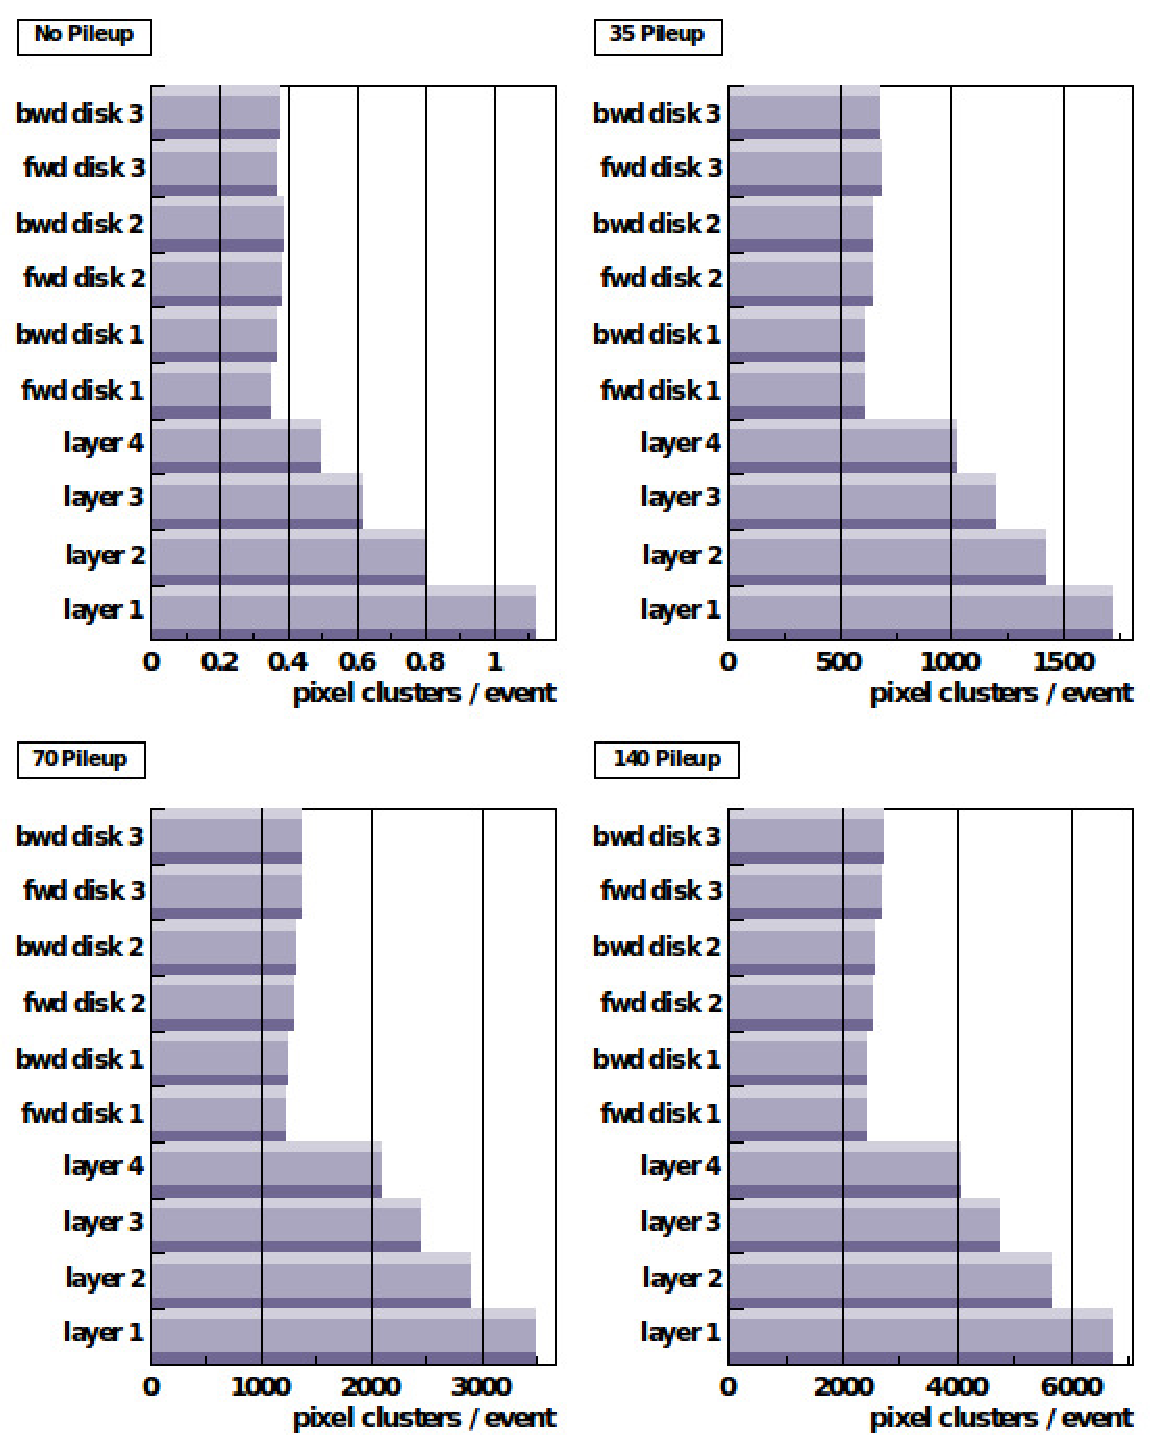
\includegraphics[scale=0.7]{Number_of_pixel_clusters.pdf}
          \caption{Number of pixel clusters per event in the different components of the pixel detector left by a single electron.
            Forward $(z>0)$ and backward $(z<0)$ disks are taken separately.}
%          \caption{Pixel clusters and ocuppancies for different pile up scenarios.}
          \label{}
        \end{figure}


%\bibliography{AngeloBib}{}
%\bibliographystyle{lucas_unsrt}
\end{document}
